\documentclass[skripsi,laporan]{itkta2025}

% ============================================================================
% KONFIGURASI IDENTITAS TUGAS AKHIR SKRIPSI
% ============================================================================
\judulid{OPTIMASI PROSES DISTILASI FRAKSINASI VAKUM DAN KRISTALISASI PATCHOULI ALCOHOL DARI MINYAK NILAM}
\judulen{OPTIMIZATION OF VACUUM FRACTIONAL DISTILLATION AND CRYSTALLIZATION OF PATCHOULI ALCOHOL FROM PATCHOULI OIL}
\penulis{Nama Mahasiswa}
\nim{11211001}
\prodi{Teknik Kimia}
\jurusan{Rekayasa Industri dan Teknologi Informasi}
\fakultas{Rekayasa dan Teknologi Industri}
\kodefakultas{FRTI}
\gelar{Sarjana Teknik (S.T.)}
\tanggal{27}
\bulan{Oktober}
\tahun{2025}
\kaprodi{Nama Koordinator Prodi, S.T., M.T.}

\pembimbingsatu{Nama Dosen Pembimbing Utama, S.T., M.T.}{199001012019031001}
\pembimbingdua{Nama Dosen Pembimbing Pendamping, S.T., M.Eng.}{199202022020121002}
\pengujisatu{Nama Dosen Penguji I, S.T., M.Sc.}{199103032018031003}
\pengujidua{Nama Dosen Penguji II, S.T., Ph.D.}{199304042021122004}

\begin{document}

% ============================================================================
% BAGIAN AWAL (Penomoran Romawi Kecil: i, ii, iii, ...)
% ============================================================================
\pagenumbering{roman}
\makecover

% Untuk Laporan TA tampilkan Orisinalitas, Publikasi, dan Pengesahan.
% Untuk Proposal TA cukup aktifkan \makepersetujuanproposal
\makeorisinalitas
\makepublikasi
\makepengeshan
% \makepersetujuanproposal % <-- Aktifkan baris ini khusus untuk Proposal TA

\frontchapter{KATA PENGANTAR}
Puji syukur kepada Tuhan Yang Maha Esa atas berkat dan anugerah-Nya sehingga penulis dapat menyelesaikan skripsi yang berjudul:
\begin{center}
  \textbf{``OPTIMASI PROSES DISTILASI FRAKSINASI VAKUM DAN KRISTALISASI PATCHOULI ALCOHOL DARI MINYAK NILAM''}
\end{center}

Laporan tugas akhir ini merupakan salah satu syarat yang harus ditempuh untuk menyelesaikan Program Sarjana di Program Studi Teknik Kimia, Jurusan Rekayasa Industri dan Teknologi Informasi, Fakultas Rekayasa dan Teknologi Industri Institut Teknologi Kalimantan (ITK) Balikpapan. Untuk itu disampaikan terima kasih yang sebesar-besarnya kepada:
\begin{enumerate}[label=\arabic*.]
  \item Bapak/Ibu Nama Dosen Pembimbing Utama, S.T., M.T. selaku Dosen Pembimbing Utama dan Bapak/Ibu Nama Dosen Pembimbing Pendamping, S.T., M.Eng. selaku Dosen Pembimbing Pendamping.
  \item Bapak/Ibu Nama Koordinator Prodi, S.T., M.T. selaku Koordinator Program Studi Teknik Kimia.
  \item Serta semua pihak yang terlibat dalam penyusunan laporan tugas akhir ini.
\end{enumerate}

Disadari bahwa penyusunan skripsi ini masih jauh dari sempurna, karena itu diharapkan segala kritik dan saran yang membangun. Semoga tugas akhir ini dapat bermanfaat bagi pengembangan ilmu pengetahuan dan teknologi. Atas perhatiannya diucapkan terima kasih.

\vspace{1.2cm}
\begin{flushright}
  Balikpapan, Oktober 2025\\[1.5cm]
  Penyusun
\end{flushright}

% ABSTRAK BAHASA INDONESIA
\begin{abstrakid}{kata kunci 1, kata kunci 2, kata kunci 3, kata kunci 4 dan kata kunci 5}
Abstrak merupakan ikhtisar suatu tugas akhir yang memuat permasalahan, tujuan, metode penelitian, hasil, dan kesimpulan. Abstrak dibuat untuk memudahkan pembaca mengerti secara cepat isi tugas akhir untuk memutuskan apakah perlu membaca lebih lanjut atau tidak. Abstrak untuk Proposal TA berisi permasalahan, tujuan dan metode penelitian, sedangkan pada Laporan TA berisi permasalahan, tujuan, metode penelitian, hasil, dan kesimpulan. Jumlah minimum kata pada abstrak adalah 200 -- 350 kata. Penulisan abstrak hanya pada satu paragraf, diketik dengan tipe font Times New Roman 12 poin dengan spasi tunggal (\textit{line spacing = single}). Setiap penggunaan bahasa asing harus diformat \textit{italic}. Format penulisan harus mengacu pada format ini.
\end{abstrakid}

% ABSTRACT BAHASA INGGRIS
\begin{abstraken}{keyword 1, keyword 2, keyword 3, keyword 4 and keyword 5}
Abstract must be in English. Abstract is a summary that contains problems, objectives, research methods for thesis proposals and contains problems, objectives, research methods, results, conclusions for thesis reports. Abstracts are made to make it easier for readers to quickly understand the contents of the final assignment to decide whether to read further or not. The minimum number of words in an abstract is 200 -- 350 words. Abstract is only one paragraph, typed in Times New Roman 12 point font with single spacing (line spacing = single).
\end{abstraken}

\makedaftarisi
\makedaftargambar
\makedaftartabel

\begin{daftarnotasi}
  $x$        & Laju alir                    & $\text{m/s}$ \\
  $y$        & Percepatan                   & $\text{m/s}^2$ \\
  $z$        & Daya                         & $\text{watt}$ \\
  $\Delta c$ & Gaya dorong supersaturasi    & $\text{g/L}$ \\
  $S$        & Rasio supersaturasi          & -- \\
\end{daftarnotasi}

% ============================================================================
% BAGIAN ISI (Penomoran Angka Arab: 1, 2, 3, ...)
% ============================================================================
\clearpage
\pagenumbering{arabic}

\chapter{PENDAHULUAN}
Pada pengantar bab ini merupakan deskripsi singkat dari isi Bab 1 Pendahuluan. Isi Bab 1 Pendahuluan meliputi: latar belakang, perumusan masalah, tujuan penelitian, manfaat penelitian, batasan penelitian, dan kerangka penelitian. Penjelasannya harus singkat, lengkap, dan dapat dimengerti oleh pembaca.

\section{Latar Belakang}
Latar belakang menyajikan konteks penelitian, untuk apa penelitian ini dilakukan, dan hal apa yang mengarahkan penelitian ini. Di sini diuraikan dalam keadaan bagaimana topik ini dilakukan.

Latar belakang memuat studi awal atau berbagai teori utama yang relevan dan baru (\textit{recent}) yang dipadukan sehingga mengerucut pada suatu persoalan unik yang kemudian disusun dalam bentuk perumusan masalah. Lazimnya bagian ini diawali dengan menguraikan kesenjangan, teoritik ataupun praktik antara harapan dan kenyataan \citep{harunsyah2021, alzoubi2023}.

\section{Perumusan Masalah}
Dalam subbab ini, permasalahan yang akan diselesaikan dirumuskan secara jelas, tajam, dan menyeluruh. Perumusan masalah dijelaskan dalam bentuk poin:
\begin{enumerate}[label=\arabic*.]
  \item Bagaimana pengaruh rasio pelarut dan suhu operasi terhadap kemurnian kristal \textit{patchouli alcohol} yang dihasilkan?
  \item Bagaimana pengaruh kecepatan pengadukan terhadap distribusi ukuran kristal (\textit{crystal size distribution})?
\end{enumerate}

\section{Tujuan Penelitian}
Pada bagian ini, tujuan dilakukannya penelitian/studi dan target atau sasaran yang ingin dicapai dinyatakan secara singkat dan jelas sesuai dengan permasalahan yang telah dirumuskan:
\begin{enumerate}[label=\arabic*.]
  \item Menentukan pengaruh rasio pelarut dan suhu operasi terhadap kemurnian kristal \textit{patchouli alcohol}.
  \item Menganalisis pengaruh kecepatan pengadukan terhadap distribusi ukuran kristal (\textit{crystal size distribution}).
\end{enumerate}

\section{Manfaat Penelitian}
Pada subbab ini dicantumkan manfaat/kegunaan khusus/dampak kemanfaatan yang diharapkan dari hasil penelitian/studi:
\begin{enumerate}[label=\arabic*.]
  \item Memberikan referensi ilmiah mengenai parameter operasi optimal pada proses kristalisasi \textit{patchouli alcohol}.
  \item Meningkatkan nilai tambah komoditas minyak nilam melalui peningkatan kemurnian produk kristal.
\end{enumerate}

\section{Batasan Penelitian}
Batasan penelitian ditetapkan untuk membantu membatasi ruang lingkup analisis dan pembahasan agar penelitian menjadi lebih fokus, terarah, dan dapat diselesaikan sesuai dengan keterbatasan waktu serta sumber daya yang tersedia.

\section{Kerangka Penelitian}
Kerangka penelitian menjelaskan \textit{state of the art} serta kaitannya dengan rencana penelitian yang diusulkan. Dengan demikian, pembaca dapat memperoleh gambaran yang jelas mengenai keterbaruan (\textit{novelty}) dari penelitian ini. Kerangka penelitian dapat disajikan dalam bentuk diagram \textit{fishbone} atau \textit{mind map}.

\chapter{TINJAUAN PUSTAKA}
Pada pengantar bab ini merupakan deskripsi singkat dari isi Bab 2 Tinjauan Pustaka. Isi Bab 2 meliputi: Pustaka/Teori I, Pustaka/Teori II, Pustaka/Teori III, dan Penelitian Terdahulu. Penjelasannya harus singkat, lengkap, dan dapat dimengerti oleh pembaca.

\section{Pustaka/Teori I}
Minyak nilam merupakan salah satu jenis minyak yang banyak dikenal oleh peneliti minyak atsiri. Berikut adalah contoh penulisan sitasi suatu penelitian dengan jumlah penulis sebanyak dua orang \citep{isfaroiny2005}. Komposisi senyawa kimia penyusun minyak nilam disajikan pada Tabel~\ref{tab:senyawa}.

\begin{table}[htbp]
  \centering
  \caption{Tabel Senyawa*)}
  \label{tab:senyawa}
  \begin{singlespace}
  \begin{tabularx}{\textwidth}{@{} >{\raggedright\arraybackslash}X l >{\centering\arraybackslash}p{3.2cm} >{\centering\arraybackslash}p{3.6cm} @{}}
    \toprule
    \textbf{Senyawa} & \textbf{Rumus Molekul} & \textbf{Berat Molekul (gr/mol)} & \textbf{Titik Didih pada 1 atm ($^\circ$C)} \\
    \midrule
    $\alpha$-Humulene           & $\text{C}_{15}\text{H}_{24}$         & 204 & 166 -- 168 \\
    $\alpha$-Copaene            & $\text{C}_{15}\text{H}_{24}$         & 204 & 246 -- 251 \\
    $\beta$-Caryophyllene oxide & $\text{C}_{15}\text{H}_{24}\text{O}$ & 220 & 279,68     \\
    Patchouli Alcohol           & $\text{C}_{15}\text{H}_{26}\text{O}$ & 222 & 287 -- 288 \\
    Pogostol                    & $\text{C}_{15}\text{H}_{26}\text{O}$ & 222 & 303 -- 304 \\
    \bottomrule
  \end{tabularx}
  \end{singlespace}
  \sumbertabel{*) \citet{aisyah2010}}
\end{table}

\section{Pustaka/Teori II}
\textit{Patchouli alcohol} atau \textit{patchoulol} merupakan senyawa utama yang terkandung dalam minyak nilam (\textit{patchouli oil}). Berikut adalah contoh penulisan sitasi suatu penelitian dengan jumlah penulis lebih dari dua orang \citep{bhatia2008}. Struktur molekul \textit{patchouli alcohol} ditunjukkan pada Gambar~\ref{fig:struktur_pa}.

\begin{figure}[htbp]
  \centering
  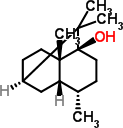
\includegraphics[width=3.8cm]{images/patchouli_struct.png}
  \caption{Struktur senyawa \textit{patchouli alcohol} \citep{berger2009}}
  \label{fig:struktur_pa}
\end{figure}

\section{Pustaka/Teori III}
Proses kristalisasi terdiri dari tiga tahapan, yaitu supersaturasi, nukleasi, dan pertumbuhan kristal. Supersaturasi merupakan \textit{driving force} dari proses kristalisasi.

\subsection{Pustaka III Bagian 1}
Banyak penelitian telah dilakukan untuk menyatakan kondisi supersaturasi. Contoh penulisan sitasi dengan lebih dari satu referensi ditulis berurutan \citep{mersmann2001a, mullin2001, jones2002, schwartz2002, tung2009}. Hubungan matematis supersaturasi dinyatakan pada Persamaan~(\ref{eq:supersaturasi}) dan Persamaan~(\ref{eq:rasio_s}):
\begin{equation}
  \Delta c = c - c^*
  \label{eq:supersaturasi}
\end{equation}
\begin{equation}
  S = \frac{c}{c^*}
  \label{eq:rasio_s}
\end{equation}

\subsection{Pustaka III Bagian 2}
Inti kristal adalah embrio pertama yang terbentuk dengan ukuran beberapa nanometer dan kemudian akan bertumbuh untuk menghasilkan kristal yang nyata.

\section{Penelitian Terdahulu}
Berikut adalah rangkuman hasil penelitian terdahulu yang memiliki keterkaitan dengan penelitian yang dilakukan sebagaimana dirangkum pada Tabel~\ref{tab:terdahulu_skripsi}. Perbandingan metode separasi juga ditampilkan pada Tabel~\ref{tab:yield_pa}.

% Tabel lintas halaman (otomatis mengulang kepala tabel jika terpotong halaman sesuai Bab 3.5.h)
\begingroup
\singlespacing\footnotesize
\begin{xltabular}{\textwidth}{@{}c p{3.5cm} X@{}}
  \caption{Penelitian Terdahulu} \label{tab:terdahulu_skripsi} \\
  \toprule
  \textbf{No.} & \textbf{Nama dan Tahun Publikasi*)} & \textbf{Hasil} \\
  \midrule
  \endfirsthead
  \multicolumn{3}{c}{\normalsize\textbf{Tabel \thetable} Penelitian Terdahulu (Lanjutan)} \\[4pt]
  \toprule
  \textbf{No.} & \textbf{Nama dan Tahun Publikasi*)} & \textbf{Hasil} \\
  \midrule
  \endhead
  \bottomrule
  \endfoot
  \bottomrule
  \multicolumn{3}{@{}l@{}}{\footnotesize *) Diurutkan sesuai tahun publikasi} \\
  \endlastfoot
  1 & \citet{su2014} & \textbf{Metode}: Distilasi fraksinasi vakum dan kristalisasi dengan pendinginan.\newline \textbf{Hasil}: Kristal \textit{patchouli alcohol} dengan kemurnian 99\% dan \textit{yield} sebesar 52,9\% serta total waktu pemisahan 7,5 jam. \\
  \addlinespace
  2 & \citet{li2021} & \textbf{Metode}: \textit{High-performance centrifugal partition chromatography} (HPCPC) dengan pelarut \textit{petroleum ether}--\textit{acetonitrile} (1:1).\newline \textbf{Hasil}: Dari 12,5 gr minyak nilam diperoleh 2 gr kristal \textit{patchouli alcohol} dengan kemurnian 98\%. \\
  \addlinespace
  3 & \citet{tong2022} & \textbf{Metode}: \textit{Host-guest inclusion} dengan senyawa \textit{host} 1,1,6,6-tetraphenylhexa-2,4-diyne-1,6-diol.\newline \textbf{Hasil}: Diperoleh kristal \textit{patchouli alcohol} sebanyak 0,102 gr (\textit{yield} kristal 17\%) dengan \textit{melting point} 81--82$^\circ$C. \\
\end{xltabular}
\endgroup

\begin{table}[htbp]
  \centering
  \caption{Perbandingan Yield dan Kemurnian Kristal PA pada Berbagai Metode Separasi}
  \label{tab:yield_pa}
  \begin{singlespace}
  \begin{tabularx}{\textwidth}{@{} l >{\centering\arraybackslash}X >{\centering\arraybackslash}X >{\centering\arraybackslash}X @{}}
    \toprule
    \textbf{Nilai} & \textbf{HPCPC *)} & \textbf{Host-Guest Inclusion \#)} & \textbf{Silica Gel Column Chrom. \$)} \\
    \midrule
    Yield  & 16\% & 17\% & 0,011\% \\
    Purity & 98\% & 44\% & 98\%    \\
    \bottomrule
  \end{tabularx}
  \end{singlespace}
  \sumbertabel{*) \citet{li2021} \\ \#) \citet{tong2022} \\ \$) \citet{xian2011}}
\end{table}

\chapter{METODE PENELITIAN}
Pada pengantar bab ini merupakan deskripsi singkat dari isi Bab 3 Metode Penelitian. Konten yang wajib ada meliputi Garis Besar Penelitian, Diagram Alir Penelitian/\textit{Flowchart}, Prosedur Penelitian, dan Variabel Penelitian.

\section{Garis Besar Penelitian}
Garis besar penelitian berisi penjelasan umum dan disusun dalam bentuk rangkuman dari metode penelitian yang digunakan.

\section{Diagram Alir Penelitian}
Tahapan pelaksanaan penelitian secara keseluruhan disajikan pada diagram alir penelitian pada Gambar~\ref{fig:flowchart_skripsi}.

\begin{figure}[htbp]
  \centering
  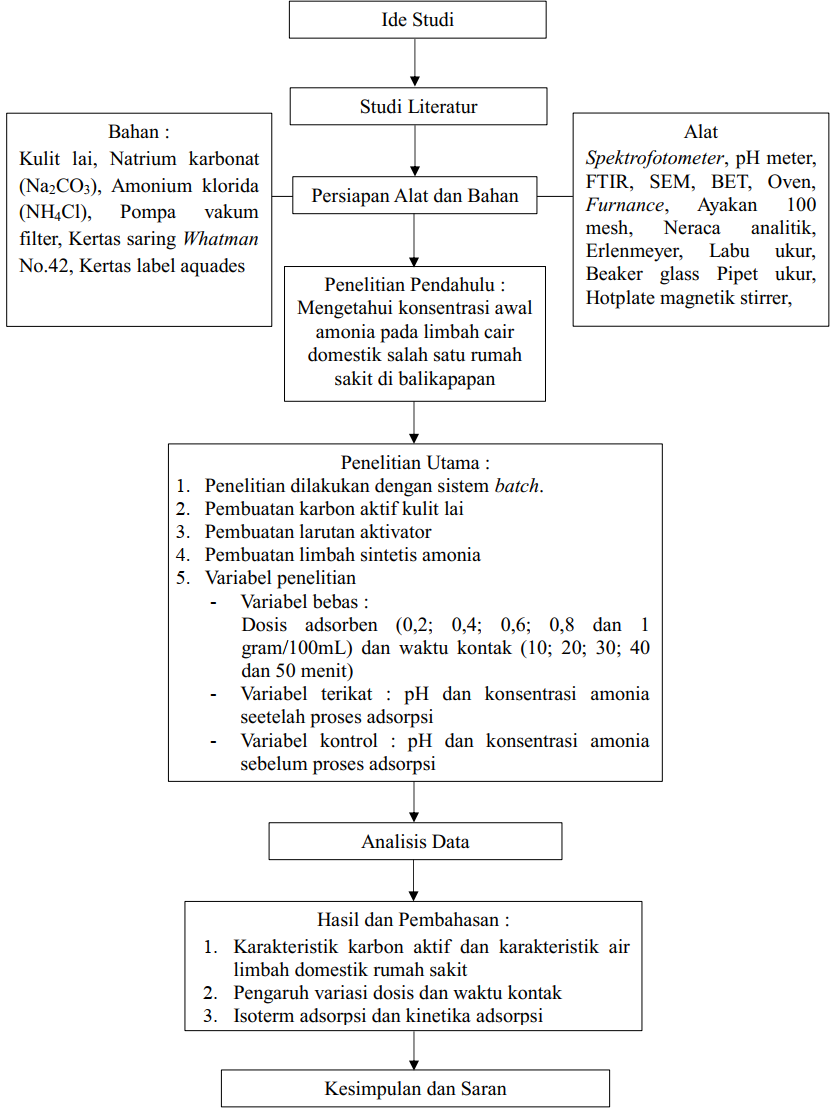
\includegraphics[width=0.78\textwidth]{images/flowchart_skripsi.png}
  \caption{Diagram alir penelitian}
  \label{fig:flowchart_skripsi}
\end{figure}

\section{Prosedur Penelitian}
\subsection{Prosedur A}
Langkah awal dalam tahap ini adalah menyiapkan bahan baku minyak nilam dan merangkai unit distilasi fraksinasi vakum sesuai kondisi operasi yang ditetapkan.

\subsection{Prosedur B}
Fraksi berat hasil distilasi selanjutnya dikristalisasi menggunakan pendinginan terkontrol dan pengadukan mekanis sesuai variasi penelitian.

\section{Variabel Penelitian}
Variabel yang digunakan dalam penelitian ini disajikan pada Tabel~\ref{tab:variabel_skripsi}.

\begin{table}[htbp]
  \centering
  \caption{Variabel Penelitian}
  \label{tab:variabel_skripsi}
  \begin{singlespace}
  \begin{tabular}{@{}p{5cm}p{6cm}@{}}
    \toprule
    \textbf{Variabel} & \textbf{Variasi Nilai} \\
    \midrule
    Kecepatan Pengadukan ($S$) & 40 rpm; 50 rpm; 60 rpm \\
    Suhu Kristalisasi ($T$)    & 5$^\circ$C; 10$^\circ$C; 15$^\circ$C \\
    \bottomrule
  \end{tabular}
  \end{singlespace}
\end{table}

\section{Rencana Jadwal Penelitian}
Rencana jadwal pelaksanaan penelitian dimulai dari seminar proposal hingga penyusunan laporan TA dan Sidang TA (subbab ini dicantumkan khusus pada dokumen Proposal Tugas Akhir).

\chapter{HASIL DAN PEMBAHASAN}
Hasil dan Pembahasan berisi hasil penelitian dan pembahasan untuk menjawab tujuan penelitian dan hipotesis. Bagian ini menyajikan data penelitian, menganalisis temuan, serta menghubungkannya dengan teori atau penelitian sebelumnya.

\section{Hasil dan Pembahasan I}
Distilasi fraksinasi merupakan proses pemisahan komponen berdasarkan perbedaan titik didih pada tekanan tereduksi \citep{mamun2008, isfaroiny2005, yudisthira2009, widiyanto2010}.

\section{Hasil dan Pembahasan II}
Kecepatan pengadukan berpengaruh signifikan terhadap distribusi ukuran kristal. Berdasarkan Gambar~\ref{fig:csd}, peningkatan kecepatan pengadukan menghasilkan distribusi ukuran kristal yang semakin \textit{unimodal}. Morfologi kristal yang dihasilkan cenderung berbentuk jarum balok dan tak beraturan (\textit{irregular}) sebagaimana ditunjukkan pada Gambar~\ref{fig:variasi_kristal}.

\begin{figure}[htbp]
  \centering
  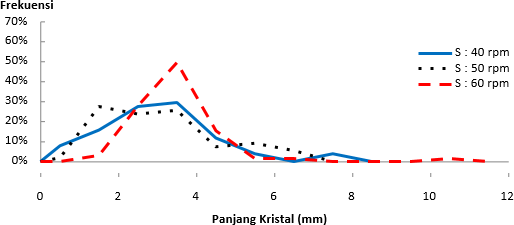
\includegraphics[width=0.78\textwidth]{images/csd_graph.png}
  \caption{\textit{Crystal size distribution} kristal \textit{patchouli alcohol}}
  \label{fig:csd}
\end{figure}

\begin{figure}[htbp]
  \centering
  \begin{subfigure}[b]{0.31\textwidth}
    \centering
    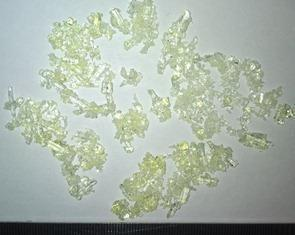
\includegraphics[width=\textwidth,height=3.4cm]{images/crystal_40rpm.jpg}
    \caption{Pengadukan 40 rpm}
  \end{subfigure}\hfill
  \begin{subfigure}[b]{0.31\textwidth}
    \centering
    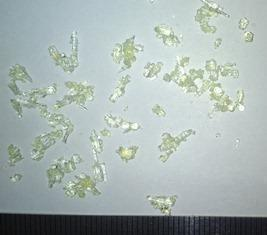
\includegraphics[width=\textwidth,height=3.4cm]{images/crystal_50rpm.jpg}
    \caption{Pengadukan 50 rpm}
  \end{subfigure}\hfill
  \begin{subfigure}[b]{0.31\textwidth}
    \centering
    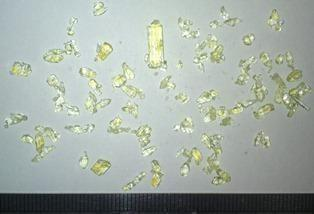
\includegraphics[width=\textwidth,height=3.4cm]{images/crystal_60rpm.jpg}
    \caption{Pengadukan 60 rpm}
  \end{subfigure}
  \caption{Variasi bentuk kristal \textit{patchouli alcohol}}
  \label{fig:variasi_kristal}
\end{figure}

\chapter{KESIMPULAN DAN SARAN}
Penutup berisi Kesimpulan dan Saran yang merangkum hasil penelitian dan memberikan rekomendasi berdasarkan temuan yang diperoleh.

\section{Kesimpulan}
Kesimpulan yang diperoleh dari hasil penelitian ini adalah:
\begin{enumerate}[label=\arabic*.]
  \item Kesimpulan pertama yang menjawab tujuan penelitian pertama secara terukur.
  \item Kesimpulan kedua yang menjawab tujuan penelitian kedua secara spesifik.
\end{enumerate}

\section{Saran}
Saran yang diperoleh dari hasil penelitian ini adalah:
\begin{enumerate}[label=\arabic*.]
  \item Dalam eksperimen distilasi fraksinasi disarankan menggunakan sistem kontrol vakum otomatis untuk menjaga kestabilan tekanan.
  \item Dalam eksperimen kristalisasi disarankan melakukan variasi laju pendinginan bertahap (\textit{stepwise cooling}).
\end{enumerate}

% ============================================================================
% BAGIAN AKHIR: DAFTAR PUSTAKA, LAMPIRAN, RIWAYAT PENULIS, & COVER BELAKANG
% ============================================================================
\clearpage
\phantomsection
\addcontentsline{toc}{chapter}{DAFTAR PUSTAKA}
\renewcommand{\bibname}{DAFTAR PUSTAKA}
\begin{singlespace}
  \bibliographystyle{itkharvard}
  \bibliography{referensi}
\end{singlespace}

\frontchapter{LAMPIRAN A}
Data mentah hasil pengamatan laboratorium dan perhitungan neraca massa disajikan pada lampiran ini.

\makeriwayatpenulis{%
\textbf{Nama Mahasiswa} lahir di Balikpapan pada 31 Januari 2003. Pada tahun 2021 terdaftar sebagai mahasiswa Institut Teknologi Kalimantan (ITK) di Program Studi S-1 Teknik Kimia. Penulis menamatkan pendidikan sekolah dasar di SD Negeri 001 Balikpapan (2009--2015), sekolah menengah pertama di SMP Negeri 2 Balikpapan (2015--2018), dan sekolah menengah atas di SMA Negeri 1 Balikpapan (2018--2021). Semasa menjadi mahasiswa ITK, penulis telah menyelesaikan penelitian tugas akhir yang berjudul ``OPTIMASI PROSES DISTILASI FRAKSINASI VAKUM DAN KRISTALISASI PATCHOULI ALCOHOL DARI MINYAK NILAM'' di bawah bimbingan Bapak/Ibu Nama Dosen Pembimbing Utama, S.T., M.T. dan Bapak/Ibu Nama Dosen Pembimbing Pendamping, S.T., M.Eng.
}

\makebackcoverandspine
\end{document}
